\section{Theorie}

\subsection{Austrittsarbeit und die Energieverteilung der Leitungselektronen}

\begin{flushleft}
    Metalle sind kristalline Festkörper, deren Kennzeichen eine hervorragende elektrische Leitfähigkeit ist.
    Die Atome die auf den Kristallgitterplätzen sitzen sind ionisiert, wobei die Ionen ein räumlich periodisches Gitter bilden mit den freigesetzten Elektronen als Hülle.
    Auf die Elektronen im Metallinneren wirkt keine Kraft und können sich somit frei bewegen, weil das Gitterpotential in grober Näherung konstant ist.
    Damit ein Elektron den Metallverband verlassen kann, muss das Elektron eine Austrittsarbeit $e_{0}\xi$ besitzen, welches gegen ein Potential $\xi$ anlaufen. 
    Die Quantentheorie liefert dabei eine Antwort auf die Frage, ob Elektronen spontan die Metalloberfläche verlassen können.
    Elektronen können nur diskrete Energiewerte annehmen.
    Diese Teilchen, mit einem halbzahligen Spin, unterliegen dem Pauli-verbot, welches besagt, dass höchstens zwei Elektronen den gleichen Energiezustand haben können, diese müssen aber einen entgegengesetzten Spin zueinander haben.
    Die Konsequenz die sich daraus ergibt ist, dass die Elektronen am absoluten Nullpunkt immer noch eine endliche Energie besitzen.
    Um die Wahrscheinlichkeit zu bestimmen, dass im thermischen Gleichgewicht ein möglicher Zustand mit der Energie E besetzt ist, wird die Fermi-Diracsche-Verteilungsfunktion verwendet.
    Aus dieser wird klar, dass für das Verlassen der Metalloberfläche die Energie des Elektrons mindestens $\xi + e_{0}\phi$ betragen muss.
    Wenn ein Elektron diese oder eine höhere Energie hat und in der Lage ist spontan die Metalloberfläche zu verlassen, kann die Fermi-Diracsche-Verteilungsfunktion genähert werden zu
\end{flushleft}

\begin{equation}
    \text{f}(\text{E}) = \text{exp}\left(\frac{\xi - \text{E}}{\text{kT}}\right)\,. \label{1}
\end{equation}

\subsection{Berechnung der Sättigungsstromdichte bei der thermischen Elektronenemission}

\begin{align}
    \intertext{Um die Sättigungstromdichte der austretenden Elektronen zu bestimmen, wird die Richardson-Gleichung verwendet.}
    \text{j}_{\text{s}}(\text{T}) = 4\pi\frac{e_{0}\,\text{m}_{0}\,\text{k}^2}{\text{h}^3}\,\text{T}^2 \text{exp}\left( \frac{-e_{0} \, \phi}{\text{kT}} \right) \label{2}
    \intertext{Diese ist abhängig von der Temperatur und und gilt bei hohen Temperaturen. } \notag
\end{align}

\subsection{Die Hochvakuum-Diode}

\begin{flushleft}
    Die Hochvakuum-Diode wird für die Messung des Sättigungsstrom einer emittierten Metalloberfläche verwendet, da die freien Elektronen sonst mit den Gasmolekülen der Luft Wechselwirken.
    Ebenso ist ein elektrisches Feld notwendig um die austretenden Elektronen abzufangen.
    In Abbildung \ref{Abbildung1} sieht man den Aufbau einer Hochvakuum-Diode, wobei diese aus einem evakuierten Glaskörper besteht, in welchem ein Draht eingeschmolzen ist.
    Dieser Draht kann durch einen Strom auf eine Temperatur von $100\,\unit{\kelvin}$ bis zu $3000\,\unit{\kelvin}$ erhitzt werden. 
    Die dabei austretenden Elektronen werden durch das erzeugte elektrische Feld abgesaugt.
\end{flushleft}

\begin{figure}[H]
    \centering
    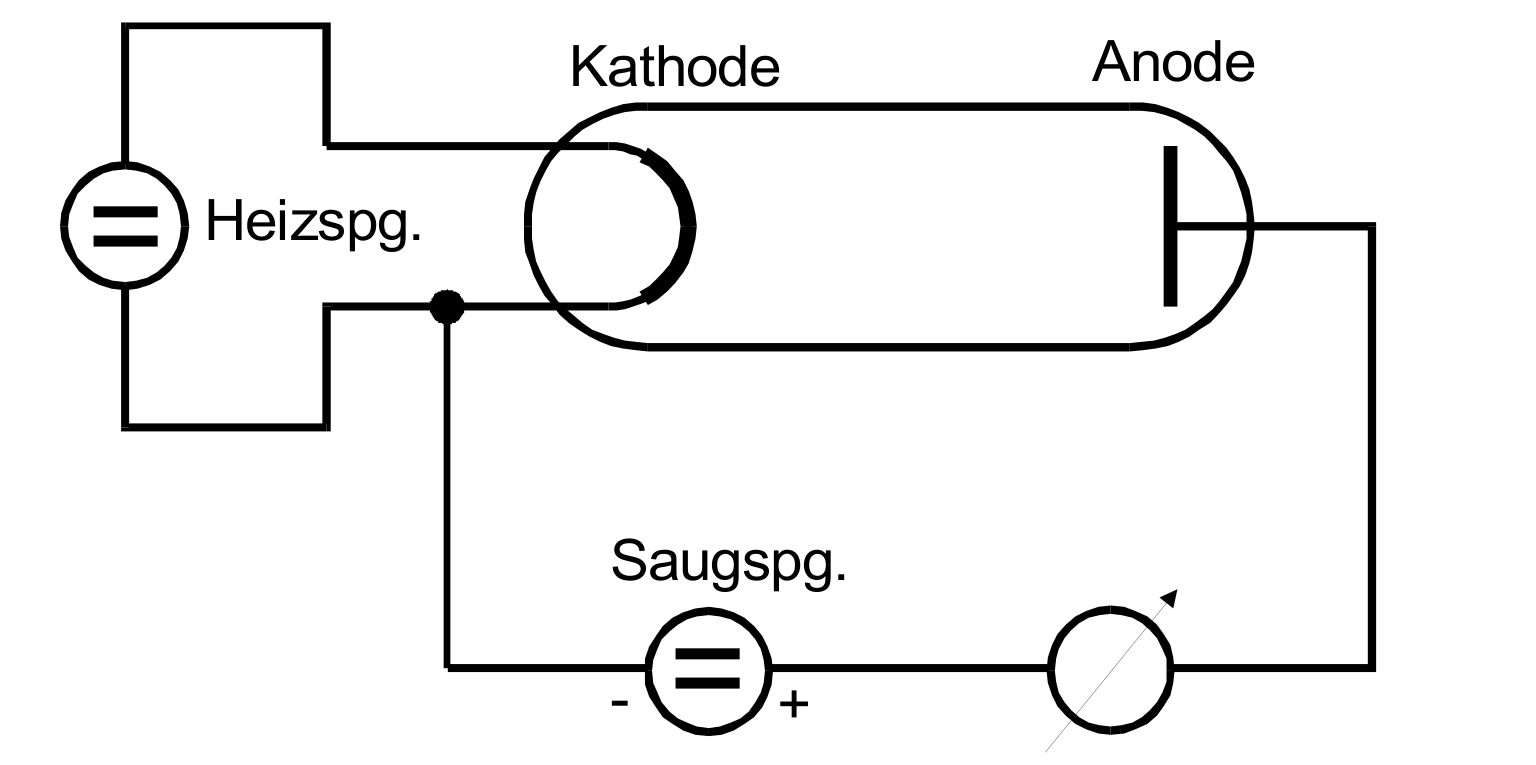
\includegraphics[height=60mm]{bilder/A1.png}
    \caption{Grundsätzliche Beschaltung einer Hochvakuum-Diode \cite{a1}. \label{Abbildung1} }
\end{figure}

\subsection{Die Langmuir-Schottkysche Raumladungsgleichung}

\begin{align*}
    \intertext{Der Anodenstrom hängt, bei gegebener Kathodentemperatur, von der Anodenspannung ab.
    Eine hinreichend hohe Anodenspannung führt zu einem Spannungs unabhängigen Strom.
    Jedoch ist das Ohmsche Gesetzt, also die Proportionalität von Strom und Spannung, auch vor Erreichen des Sättigungswertes bei einer Diode ungültig.
    Grund dafür ist, dass die Geschwindigkeit der Elektronen nicht mehr konstant ist und dies dazu führt, dass die Raumladungsdichte $\rho$ eine Funktion des Ortes wird und in Richtung der Anode abnimmt.}
    \text{j} = - \rho \cdot \text{v}
    \intertext{Der Verlauf der Feldstärke zwischen Anode und Kathode wird durch die Raumladungsdichte beeinflusst, weil diese das Feld von der Kathode abschirmt.
    Die Feldlinien die von der Anode ausgehen reichen nicht mehr bis zur Kathode und enden schon an den Raumladungselektronen.
    Die emittierten Elektronen werden dann nicht mehr als von dem Anodenfeld erfasst, wodurch der gemessene Diodenstrom kleiner als der Sättigungsstrom ist.
    Dargestellt wird dies durch das Langmuir-Schottkysche Raumladungsgesetz, wobei der Gültigkeitsbereich dieser auch Raumladungsgebiet genannt wird}
\end{align*}

\begin{equation}
    \text{j} = \frac{4}{9} \, \varepsilon_{0}\, \sqrt{ \frac{2\,e_{0}}{\text{m}_{0}} }\, \frac{\text{V}^{\frac{3}{2}}}{\text{a}^2}\,. \label{3}
\end{equation}

\subsection{Das Anlaufstromgebiet einer Hochvakuumdiode}

\begin{flushleft}
    Aus der Gleichung (\ref{3}) folgt, dass bei $\text{V} = 0$ auch $\text{j} = 0$ ist.
    Jedoch wird beobachtet das bei $\text{V} = 0$ noch ein geringer Anodenstrom vorhanden ist.
    Dieser entsteht durch die Eigengeschwindigkeit der Elektronen beim Verlassen der Kathode. 
    Bei $\text{T} > 0$ sind endlich viele Elektronen mit der Energie größer als die der Austrittsarbeit, welche gegen ein geringer Anlaufstrom anlaufen können, wobei das Anodenmaterial die Austrittsarbeit $\phi_{\text{A}}$ besitzt.
    Dadurch müssen die Elektronen, die die Anode erreichen, eine größere Energie besitzen als $e_{0}\,\phi_{\text{A}} + e_{0}\,\text{V}$.
    Beschrieben wir der Verlauf des Anodenstromgebietes durch
\end{flushleft}

\begin{align}
\text{j}(\text{V}) = \text{j}_{0}\, \text{exp} \left(- \frac{e_{0}\,\phi_{\text{A}} + e_{0}\, \text{V} }{\text{kT}}\right) = \text{const}\,\, \text{exp} \left(\frac{e_{0}\, \text{V}}{\text{kT}} \right) \,. \label{4}
\end{align}

\subsection{Die Kennlinie der Hochvakuumdiode}

\begin{flushleft}
    Die Kennlinie einer Hochvakuumdiode stellt den Zusammenhang zwischen der Stromdichte j bzw. dem Anodenstrom $\text{I}_{\text{A}}$ und dem außen angelegten Potential dar.
    Einteilen lassen sich diese Kennlinien in drei Gebiete, wie in Abbildung \ref{Abbildung2} zu sehen.
    Das erste Gebiet ist das Anlaufstromgebiet, in welchem der Zusammenhang zwischen I und V im Bereich $\text{V} > 0$ existiert.
    Das zweite Gebiet ist das Raumladungsgebiet, in welchem die $\sqrt{\text{V}^3}$-Abhängigkeit vorhanden ist.
    Für die Bestimmung der Kathodentemperatur und der Austrittsarbeit der Kathode können teile der Kennlinie benutzt werden.
\end{flushleft}

\begin{figure}[H]
    \centering
    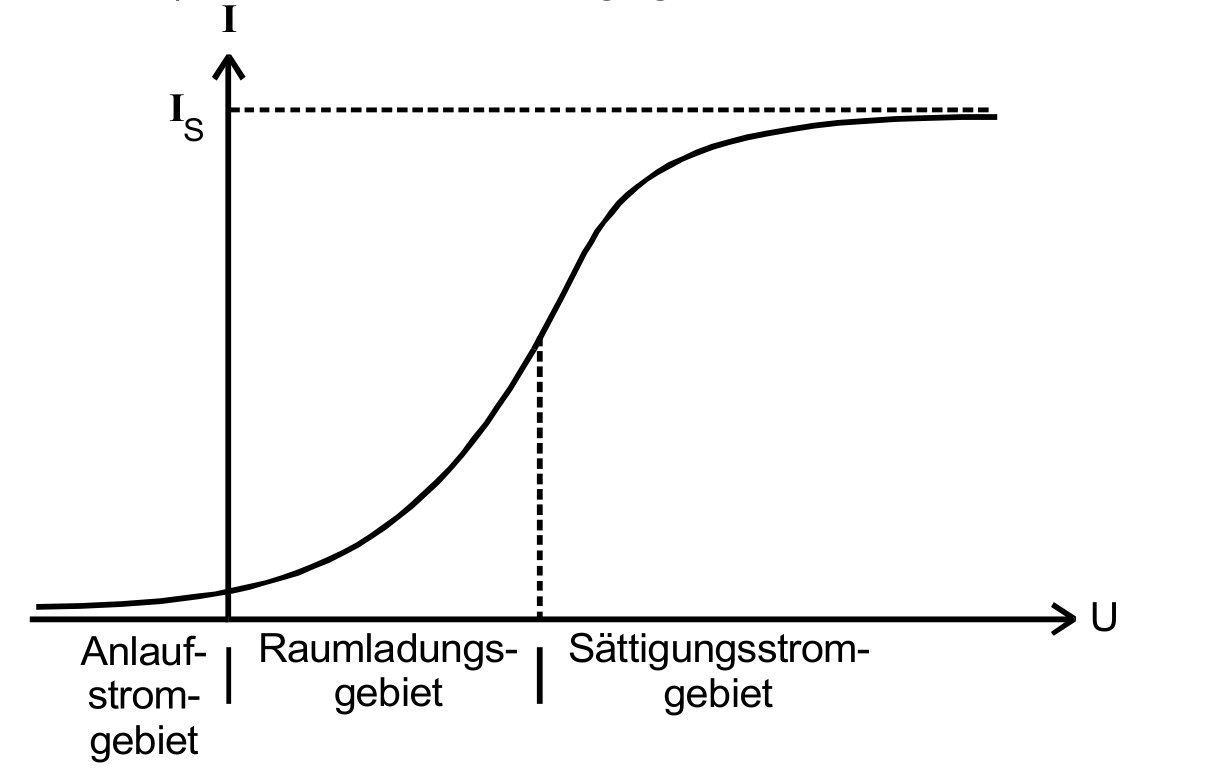
\includegraphics[height=70mm]{bilder/A2.png}
    \caption{Kennlinie einer Hochvakuumdiode \cite{a1}. \label{Abbildung2} }
\end{figure}
